\documentclass[12pt]{article}
\usepackage{graphicx}
\usepackage[latin1]{inputenc}
\author{Joao Vitor Elias Carvalho - 112037860}
\title{Trabalhando com Grandes Volumes de Dados}

\begin{document}
\maketitle

\newpage

\newpage

\section{ Pergunta }

Qual melhor tipo de pokemon baseado em qual tipo tem vantagem sobre outro tipo. Basicamente qual tipo possui mais pokemons que ele tem vantagem dentro desse dataset.

\section{ Dados }

Vamos utilizar o dataset composto pelos 721 pokemons retirados do site Kaggle. Alem disso foi necess�rio introduzir as vantagens e desvantagens de em rela��o a cada tipo de pok�mon. Ap�s uma pesquisa, achei a tabela de Strengths e Weakness que transformei em um arquivo JSON para ser utilizado facilmente no c�digo.

\section{ M�todo } 

Utilizei a linguagem Python. As bibliotecas utilizadas foram: csv, json, numpy e matplotlib. Primeiramente contabilizei quantos pokemons de cada tipo existiam no database guardando-os em um dicion�rio. Ent�o utilizando a tabela de strengths e weakness eu percorrei cada tipo somando quantos pokemons aquele tipo possu�a vantagem ou desvantagem. Ap�s isso foi s� uma quest�o de plotar as informa��es em um gr�fico de barra.

\section{ Resultados }

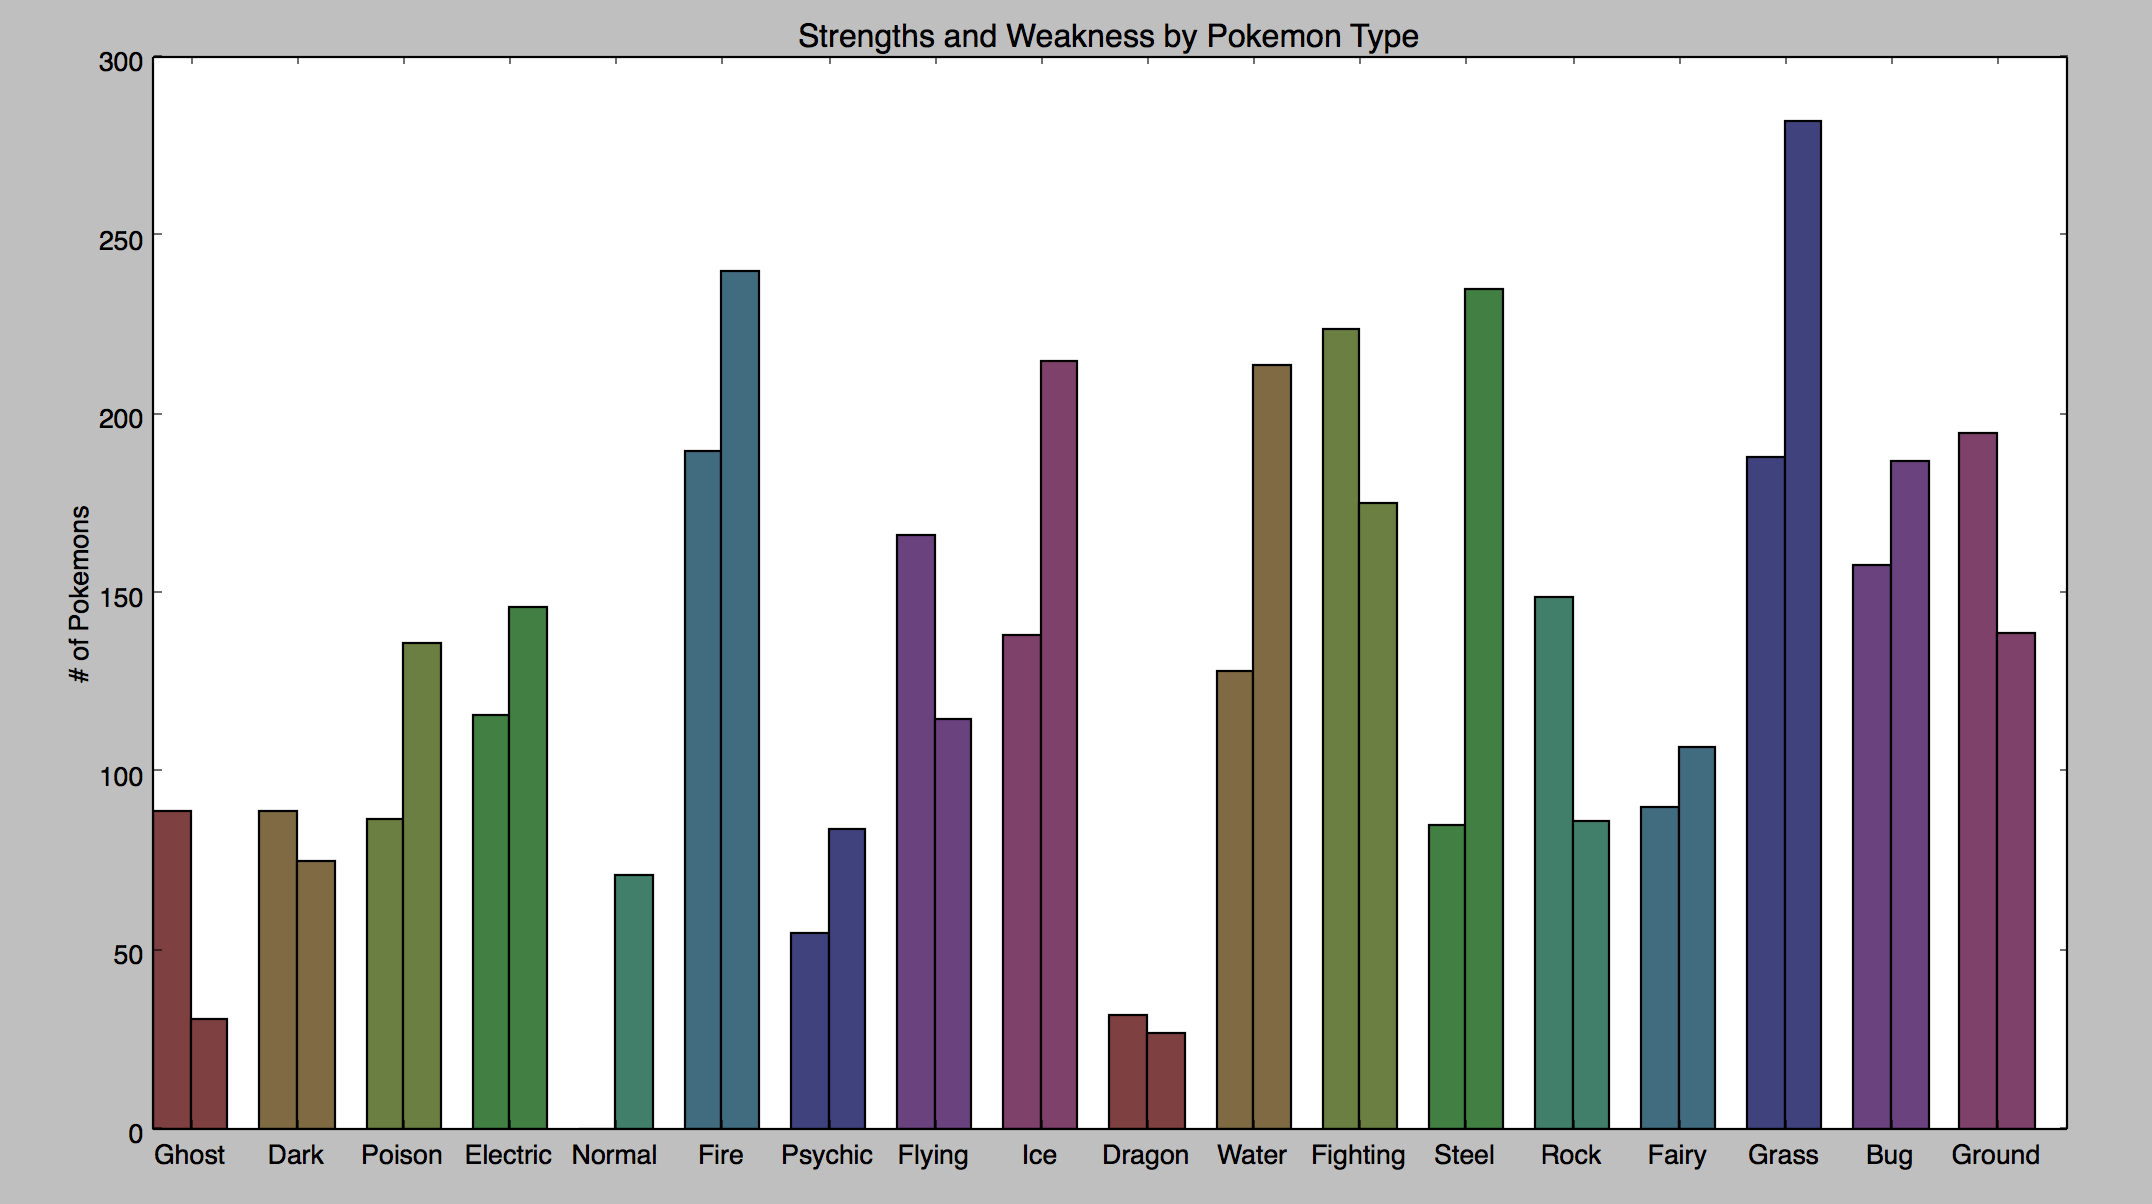
\includegraphics[width=\textwidth]{graph.png}

Cada tipo possui duas barras: a primeira � a contagem de quantos pokemons ele possui vantagem e a segunda � quantos pokemons ele possui desvantagem. 

Podemos observar alguns tipo que possuem mais vantagens do que desvantagens como o tipo Fighting, Ghost, Rock e Ground.


\end{document}